\chapter{DCF controller}
\section{Inleiding}
De basis van onze wekker wordt gelegd door een klok. Uit dit onderdeel, genaamd DCF-controller,  komt verschillende data, als de tijd, de datum en het weeknummer. Een van de eigenschappen van deze klok zal zijn dat hij gesynchroniseerd wordt met een zogenaamd DCF-signaal. Dit is een signaal dat in duitsland verzonden wordt en allerlei informatie bevat, als de actuele tijd en de datum. Er zullen meerdere van deze elementen gebruikt worden in onze wekker.  Al deze data wordt verzonden door middel van een pulssignaal. Vanuit Duitland wordt elke seconde een puls van 100 of 200 ms verstuurd, zodat respectievelijk een 0-bit en een 1-bit doorgegeven wordt. Dit resulteert in een totaal van 59 bits, gevolgt door een seconde ‘rust’, dat elke minuut opnieuw verzonden wordt. In figuur \ref{fig:Blokdiagram} is te zien welke secondes welke informatie bevatten. In de afbeelding wordt een aantal keer P\# genoemd. Dit zijn paritychecks om het ingekomen signaal te controleren. Als de voorgaande bits een even aantal logische enen bevat, zal de parity bit een logische 0 geven. ~\cite{Tijdscodering} \emph{\color{red} \#\# Controleren \#\#} De controller converteert dit gedigitaliseerde DCF77 signaal naar een tijdreferentie, waarna deze een autonome klok synchroniseert, welke de huidige tijd genereerd.

\begin{figure}[h!]
\center
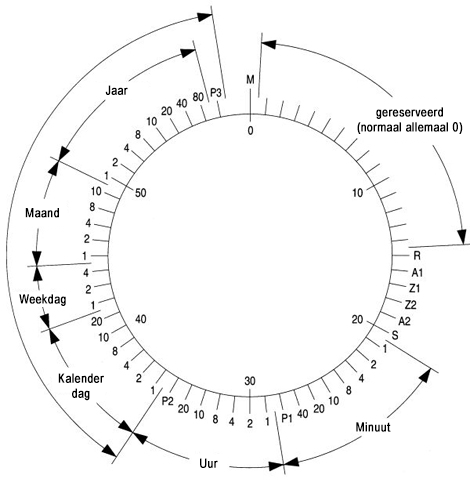
\includegraphics[scale=2]{Figuren/DCF77/dcf77coding.png}
\caption{Codering van het dcf-signaal~\cite{Tijdscodering}}
\label{fig:dcfsignaal}
\end{figure}

\section{Specificaties}
In deze sectie zullen we de in- en uitgangen van de DCF-controller in een overzicht weergeven. Doordat het totale systeem met dit onderdeel start, bevat dit blok enkel standaard ingangen en een ingang van buitenaf. De uitgangen uren en minuten worden doorgestuurd naar de main-controller. De clk van 1 Hz zal in verschillende onderdelen worden gebruikt. De debug\_led zal rechtstreeks op het LCD worden weergegeven. 
\subsection{Ingangen}
Dit onderdeel maakt gebruik van de volgende ingangen: 

\begin{itemize}[nolistsep]
\item Reset, standaard input.
\item Klok, standaard input.
\item DCF, signaal van 'logische' pulsen.
\end{itemize}
\noindent

\subsection{Uitgangen}
Dit onderdeel heeft de volgende uitgangen:
\begin{itemize}[nolistsep]
\item Uren, een BCD vector van 6 bits.
\item minuten, een BCD vector van 7 bits.
\item clk, een clk die elke seconde een puls geeft.
\item debug\_led, een signaal dat een logische 1 doorgeeft zodra er een dcf signaal wordt ontvangen.
\end{itemize}


\section{Gedrag}
De DCF-controller heeft als belangrijkste gedragsfunctie om de tijd en datum door te geven. Al deze data moet zo vaak mogelijk worden gesynchroniseerd met een inkoment DCF-signaal. Dit signaal moet vanaf een antenne gedecodeerd worden en vervolgens moet het signaal via parity bits gecontroleerd worden. Pas als hieraan voldaan is moet het signaal in een register worden geschreven en doorgestuurd naar de andere onderdelen van de chip. Mocht het DCF-signaal signaal niet of slecht worden ontvangen dan moet de tijd instantaan en individueel door kunnen lopen. Indien het DCF-signaal weer terugkomt moet de controller dit automatisch oppakken. Om aan te geven of er een  DCF signaal is, moet er een zogenaamd debug lampje gaan branden als dit gebeurt. In de 60e seconde zal dit signaal laag moeten zijn, doordat dan geen bit doorgegeven wordt. \\
De huidige, indien mogelijk met het DCF77 signaal gesynchroniseerde, tijd moet worden gegeven in uren (in een BCD gecodeerd signaal van 5-bits) en minuten (in een BCD gecodeerd signaal van 6-bits). De datum, afkomstig uit het DCF77 signaal dient na synchronisatie te worden bewaard totdat er opnieuw met het DCF77 signaal wordt gesynchroniseerd. De datum wordt gegeven in vier vectoren:
\begin{itemize}[nolistsep]
\item De dag van de week wordt gegeven door drie bits, waarbij maandag is gecodeerd als 001, dinsdag als 010, enz.
\item De dag van de maand, gegeven als BCD gecodeerd signaal van 6-bits.
\item Het nummer van de maand wordt gegeven als BCD gecodeerd 5-bits signaal.
\item De laatste twee cijfers van het huidige jaartal worden bovendien gegeven door een 8-bits BCD gecodeerd signaal.
\end{itemize}
\vspace{0.3cm}
Daarnaast moet de DCF-controller ook een 1 Hz kloksignaal via een klokdeler naar alle andere onderdelen kunnen sturen.
Als laatste moeten alle subblokken, inclusief registers, van de DCF-controller bij een 'active high' van een resetknop gereset worden.